\chapter{Méthode d'ordre élevé pour le suivi d'un carreau de surface}%patch surfacique rectangulaire}
\label{chap:methode_ps}

\textit{on veut mettre au point une méthode numérique (discrétisations spatiale et temporelle) pour le suivi d'un seul patch rectangulaire de surface de continuité géométrique élevée (infinie), qui servira de base pour  mettre en \oe uvre l'algorithme du \autoref{chap:algo_general}}
\par\bigskip

suivi lagrangien de marqueurs/points de collocation situés sur la surface

\section{Discrétisation spectrale en espace}%spatiale}
méthode pseudo-spectrale : solution développée dans une base de fonctions globales et régulières, résidu annulé exactement en un nombre discret de points de collocation, donnant une EDO en temps par point de collocation\par
Choix des fonctions de base et des marqueurs/points de collocation\par

\subsection{État de l'art}
Le choix des fonction de base se pose alors. Celles-ci doivent pouvoir représenter n'importe quel type de solution avec une précision arbitraire, offrir une convergence rapide à mesure que le nombre de degrés de liberté augmente et enfin pouvoir être évaluées efficacement. A ces critères s'ajoutent également des contraintes liées à la topologie de la solution (i.e. l'interface en propagation).\par

Traditionnellement, les méthodes spectrales reposent sur les séries de Fourier lorsque la solution est spatialement périodique. 
Les polynômes trigonométriques ont ainsi été utilisés comme fonctions de base pour représenter un front de flamme dans une configuration quasi-3{\scshape d} \cite{gueyffier2015} (\textbf{reformuler}).
Lorsque la solution est une surface fermée de genre zéro (\ie une sphère topologique), la base des harmoniques sphériques est particulièrement adaptée \cite{veerapaneni2011}.\par
Les travaux de Bruno \cite{bruno2007} sur une méthode de \eng{continuation} ont permis d'étendre l'usage des polynômes trigonométriques aux surfaces homéomorphes à des disques. 
Cette approche permet de représenter des surfaces de géométrie complexe et de topologie arbitraire en raccordant des patchs locaux à l'aide de partitions de l'unité.\\
\textbf{Permet d'éviter Gibbs dans le cas régulier par morceaux}\\
A l'instar de la méthode proposée dans cette thèse, l'idée est alors de représenter des surfaces de géométrie complexe et de topologie arbitraire à l'aide de paramétrisations locales en construisant un atlas. 
En revanche, cette approche nécessite la résolution de systèmes linéaires mettant en jeu des matrices de grande taille, pleines et généralement mal conditionnées. 
En outre, cette méthode n'a à ce jour pas été appliquée pour la déformation de surface.
%Ce type de discrétisation spectrale a notamment été utilisé pour la représentation de vésicules inextensibles en suspension dans un écoulement fortement visqueux \cite{veerapaneni2011}. 
%Dans ces travaux, la base des harmoniques sphériques est naturellement adaptée à la topologie des vésicules (genre 0 sans bord).
%Les polynômes trigonométriques ont également été utilisés comme fonctions de base pour représenter un front de flamme une configuration quasi-3{\scshape d} \cite{gueyffier2015}.

\begin{itemize}
	\item harmoniques sphériques \cite{veerapaneni2011}, polynômes trigonométriques \cite{gueyffier2015} $\to$ contraintes topologiques (genre 0, sans bord ou périodique) (méthode de continuation \cite{bruno2007} pour s'affranchir de cette contrainte, mais complexe (POUs, \ldots) et jamais utilisé pour des surfaces en mouvement)
	\item CAO : courbes/surfaces polynomiales (algébriques)/rationnelles (en produit tensoriel) par morceaux (B-splines/NURBS), utilisant la base de Bernstein
	\begin{equation}
		B_n^N(x) = \binom{N}{n} \left( 1 - x \right)^{N-n} x^n.
	\end{equation}
	\begin{itemize}
		\item[+] coefficients = points de contrôle dans l'espace physique, sens géométrique intuitif
		\item[+] partition de l'unité sur $\berninterval$ $\Rightarrow$ propriété d'enveloppe convexe
		\item[-] algorithme d'évaluation (de Casteljau) numériquement stable mais coûteux $\bigO{N^2}$
		\item[-] points de contrôle pas \emph{sur} la courbe/surface $\Rightarrow$ pas exploitables comme marqueurs lagrangiens
		\item[-] peu pratiques pour réduire/élever le degré des polynômes
	\end{itemize}
\end{itemize}
\bigskip
on choisit les polynômes de Chebyshev, couramment employés dans les méthodes spectrales dans le cas non-périodique
%on choisit les polynômes de Chebyshev\footnotemark, couramment employés dans les méthodes spectrales dans le cas non-périodique
%\footnotetext{En français, le nom de ce mathématicien russe est généralement orthographié \guill{Tchebychev}. Nous utiliserons cependant l'orthographe anglo-saxone, plus couramment utilisée par la communauté scientifique.}
%(Mason, p.81) >>>-----
%Orthogonal polynomials have a great variety and wealth of properties,
%many of which are noted in this chapter. Indeed, some of these properties
%take a very concise form in the case of the Chebyshev polynomials, making
%Chebyshev polynomials of leading importance among orthogonal polynomi-
%als — second perhaps to Legendre polynomials (which have a unit weight
%function), but having the advantage over the Legendre polynomials that the
%locations of their zeros are known analytically. Moreover, along with the Legendre polynomials, the Chebyshev polynomials belong to an exclusive band
%of orthogonal polynomials, known as Jacobi polynomials, which correspond
%to weight functions of the form (1 − x) α (1 + x) β and which are solutions of
%Sturm–Liouville equations.
%The Chebyshev polynomials have further properties, which are peculiar
%to them and have a trigonometric origin, namely various kinds of discrete
%orthogonality over the zeros of Chebyshev polynomials of higher degree. In
%consequence, interpolation at Chebyshev zeros can be achieved exceptionally
%inexpensively (Chapter 6) and Gauss quadrature methods based on Cheby-
%shev zeros are extremely convenient (Chapter 8).
%<<<-----



\subsection{Polynômes de Chebyshev}
Les polynômes de Chebyshev sont très largement utilisés dans de nombreux domaines tels que l'analyse numérique.
L'objet des sections suivantes est de rappeler la définition de cette famille 
de polynômes et d'en présenter brièvement les propriétés remarquables qui seront exploitées dans cette thèse. 
Nombreux sont les ouvrages consacrés aux polynômes de Chebyshev \cite{mason2002, gil2007} ainsi qu'à leur usage dans les méthodes spectrales \cite{boyd2001, canuto2006}, aussi le lecteur est invité à s'y référer pour plus de détails.


\subsubsection{Définition et propriétés}
\begin{definition}
	Pour $n \in \mathbb{N}$, le polynôme de Chebyshev (de première espèce) $T_n$ est défini par%un polynome de degré $n$ défini par
	\begin{equation}
		T_n(\cos \theta) = n \cos \theta.
		\label{eq:chebyshev_trigo}
	\end{equation}
\end{definition}
%De la définition \eqref{eq:chebyshev_trigo} et de l'identité trigonométrique
De cette définition et de l'identité trigonométrique $\cos n\theta + \cos (n-2)\theta = 2\cos \theta \cos (n-1)\theta$, on peut déduire la relation de récurrence suivante, pour $x \in \chebinterval$, 
\begin{align}[left = \empheqlbrace\,]
	T_0(x) &= 1, \nonumber\\
	T_1(x) &= x, \nonumber\\
	T_n(x) &= 2x T_{n-1}(x) - T_{n-2}(x) \text{,\ pour\ } n \geq 2.
	\label{eq:chebyshev_recurrence}
\end{align}
Le graphe des six premiers polynômes de Chebyshev est tracé sur la \autoref{fig:chebyshev_polynomials}.\par

\begin{figure}
	\centering
	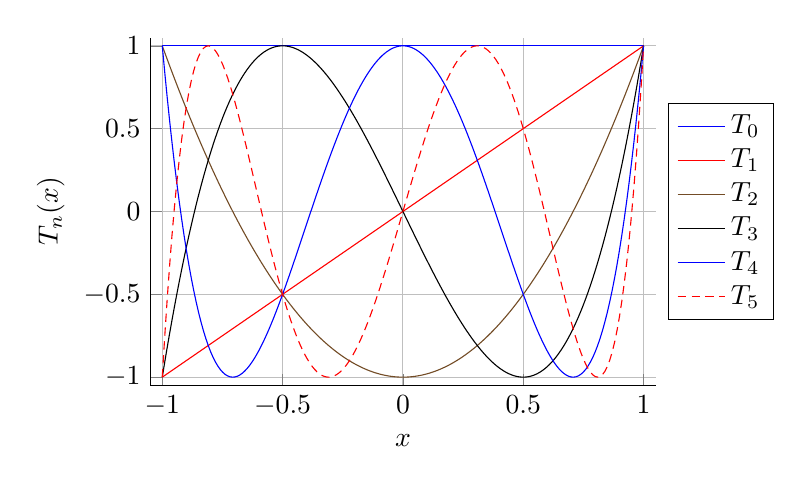
\begin{tikzpicture} 
	\begin{axis}[%
		width=8cm, height=6cm,
		axis lines*=left,
		xmin=-1.0, xmax=1.0, ymin=-1.0, ymax=1.0,
		grid=major,
		clip marker paths=false,
		enlargelimits={abs=0.05},
		xlabel={$x$},
		ylabel={$T_n(x)$},
		legend style={at={(1.025,0.5)}, anchor=west},
		no marks,
		samples=200
		]%
		\addplot+[domain=-1:1] {1.0};%
		\addplot+[domain=-1:1] {x};%
		\addplot+[domain=-1:1] {2.0*x^2 - 1.0};%
		\addplot+[domain=-1:1] {4.0*x^3 - 3.0*x};%
		\addplot+[domain=-1:1] {8.0*x^4 - 8.0*x^2 + 1.0};%
		\addplot+[domain=-1:1] {16.0*x^5 - 20.0*x^3 + 5.0*x};%
		\legend{{$T_0$},{$T_1$},{$T_2$},{$T_3$},{$T_4$},{$T_5$}}%
	\end{axis} 
\end{tikzpicture}
	\caption{Graphe des premiers polynômes de Chebyshev.}% $(n=0,\ldots,5)$ sur l'intervalle $\chebinterval$.}
	\label{fig:chebyshev_polynomials}
\end{figure}

%\begin{figure}
%	\centering
%	\begin{tikzpicture}
%		\begin{axis}[
%			width=12cm, height=9cm,
%		    set layers=standard,
%		    domain=-1:1,
%		    xmin=-1, xmax=1,
%		    zmin=-1, zmax=1,
%		    samples y=1,
%		    view={40}{30},
%		    grid = major,
%		    axis lines* = left,
%		    unit vector ratio*=4 3 1,
%		    xtick={-1,-0.5,0,0.5,1},
%		    ytick={0,1,2,3,4,5},
%		    ztick={-1,0,1},
%		    xlabel={$x$},
%		    ylabel={$n$},
%		    zlabel={$T_n(x)$},
%		    no marks,
%		    samples=201,
%		    every tick label/.append style={font=\small},
%		    %tick align=outside,
%		%    cycle list/GnBu-9,%RdYlBu-6,%Spectral-6,
%		%	cycle multiindex* list={GnBu-9},%RdYlBu-6}%Spectral-6}
%		    clip=false]
%			\pgfplotsinvokeforeach{0,1,...,5}{%
%				\addplot3+[domain=-1:1]	({x},#1,{ cos(#1*acos(x)) });
%			}%
%		\end{axis}
%	\end{tikzpicture}
%	\caption{Graphe des premiers polynômes de Chebyshev.}
%\end{figure}
%
%\begin{figure}
%	\centering
%	\begin{tikzpicture} 
%		\begin{axis}[%
%			width=8cm, height=6cm,
%			axis lines*=left,
%			xmin=-1.0, xmax=1.0, ymin=-1.0, ymax=1.0,
%			grid=major,
%			clip marker paths=false,
%			enlargelimits={abs=0.05},
%			xlabel={$x$},
%			ylabel={$T_n(x)$},
%			legend style={at={(1.025,0.5)}, anchor=west},
%			no marks,
%			samples=201,
%			%cycle list/GnBu-9,%RdYlBu-6,%Spectral-6,
%			%cycle multiindex* list={GnBu-9}%RdYlBu-6}%Spectral-6}
%			]%
%			\pgfplotsinvokeforeach{0,1,...,5}{%
%	      		\addplot+[domain=-1:1] { cos(#1*acos(x)) } coordinate[pos=0.8+#1*0.011] (x#1);
%%	      		\pgfmathparse{0.75}\let\xa\pgfmathresult
%%	      		\pgfmathparse{cos(#1*acos(0.75))}\let\ya\pgfmathresult
%%	      		\pgfmathparse{0.75-#1*0.25}\let\yb\pgfmathresult
%	      		%\def\xa{\pgfmathparse{0.75}\pgfmathresult}
%	      		%\def\ya{\pgfmathparse{cos(#1*acos(\xa))}\pgfmathresult}
%	      		%\xdef\ya{1.0 - #1*0.15}
%	      		%\xdef\xa{cos(acos(\ya)/#1)}
%	      		%\def\yb{\pgfmathparse{0.75-#1*0.25}\pgfmathresult}
%	        	%\addlegendentry{$T_{#1}$}
%	        	\draw[latex-, black, thin] 
%	        		(x#1)
%	        		to [bend right=20] 
%	        		(axis cs:1.1,1-2*#1/5) 
%	        		node [anchor=west] {$n=#1$};
%	        }%
%		\end{axis} 
%	\end{tikzpicture}
%	\caption{Graphe des premiers polynômes de Chebyshev $(n=0,\ldots,5)$ sur l'intervalle $\chebinterval$.}
%%	\label{fig:chebyshev_polynomials}
%\end{figure}

%En posant $x = \cos \theta$, il vient
%\begin{equation}
%	\dfdx{T_n(x)}{x} = \frac{n \sin n\theta}{\sin \theta}.
%\end{equation}

$T_n$ est un polynôme de degré $n$ %de coefficient dominant $2^{n-1}$ 
qui atteint ses extrema locaux sur $\chebinterval$ aux $n+1$ n\oe uds de Chebyshev-Gauss-Lobatto (CGL)%\footnote{Seuls les $n-1$ n\oe uds intérieurs sont réellement des extrema au sens où la dérivée s'y annule. A noter également que ces n\oe uds sont rangés en ordre décroissant.}
\begin{equation}
	x_k = \cos \frac{k \pi}{n},
	\label{eq:cgl_nodes}
\end{equation}
pour $0 \leq k \leq n$. 
Seuls les $n-1$ n\oe uds intérieurs sont réellement des extrema au sens où la dérivée s'y annule. 
A noter également que ces n\oe uds sont rangés en ordre décroissant.\par
Comme illustré sur la \autoref{fig:cgl_nodes}, ces extrema sont alternativement des maxima puis des minima, tous égaux en valeur absolue
\begin{equation}
	T_n(x_k) = (-1)^{k}.
	\label{eq:chebyshev_equioscillation}
\end{equation}

\begin{figure}
	\centering
	\begin{tikzpicture} 
	\begin{axis}[%
		width=8cm, height=6cm,
		axis lines*=left,
		xmin=-1.0, xmax=1.0, ymin=-1.0, ymax=1.0,
		grid=major,
		clip marker paths=false,
		enlargelimits={abs=0.05},
		]%
		\addplot+[samples=200, domain=0:pi, no marks, s6] ({cos(deg(x))}, {cos(5*deg(x))});%
		% extrema
		\addplot+[samples=6, domain=0:pi, ycomb, dashed, mark=none, black] ({cos(deg(x))}, {cos(5*deg(x))});%
		\addplot+[samples=6, domain=0:pi, only marks, mark=*, black] ({cos(deg(x))}, {0});%
		% zeros
%		\pgfplotsinvokeforeach{0,...,4}{
%			\addplot+[mark=*, red] coordinates {(cos((2.0*#1+1.0)*180.0/10.0),0)};
%		}
	\end{axis} 
\end{tikzpicture}
%	\caption{N\oe uds de Chebyshev-Gauss-Lobatto pour $n = 6$ (extrema locaux du polynome $T_6$ sur l'intervalle $\chebinterval$).}
	\caption{N\oe uds de Chebyshev-Gauss-Lobatto (extrema locaux) du polynôme $T_5$.}% sur l'intervalle $\chebinterval$.}
	\label{fig:cgl_nodes}
\end{figure}

%Cette propriété dite d'\emph{équioscillation} a pour conséquence --- via un théorème attribué au mathématicien Émile Borel --- que la meilleure approximation uniforme (\ie en norme $L_\infty$) polynomiale de degré $n - 1$ de la fonction $x \mapsto x^n$ sur $\chebinterval$ est la fonction $x \mapsto x^n - 2^{1 - n} T_n(x)$. \\
%$\to$ économisation\ldots
Cette propriété d'\emph{équioscillation} a pour conséquence le théorème suivant.
\begin{theoreme}
	Le polynôme %$p_{N-1}$ 
	de degré $N-1$ qui donne la meilleure approximation uniforme (\ie en norme $L_\infty$) %de la fonction $x \mapsto x^N$ est $p_{N-1} : x \mapsto x^N - 2^{1 - N} T_n(x)$. 
du polynôme %$q : x \mapsto \sum_{n=0}^{N} a_n x^n$
$q = \sum_{n=0}^{N} a_n X^n$ 
sur l'intervalle $\chebinterval$ est
	\begin{equation}
		p_{N-1} = q - 2^{1-N} a_N T_N,
	\end{equation}
	et, pour tout $x \in \chebinterval$,
	%La meilleure approximation %uniforme (\ie en norme $L_\infty$) 
	%polynomiale de degré $N - 1$ en norme $L_\infty$ de la fonction $x \mapsto x^N$ sur $\chebinterval$ est la fonction $p_N : x \mapsto x^N - 2^{1 - N} T_n(x)$ et
	\begin{equation}
		%\norminf{q - p_{N-1}} = 2^{1-N} \left| a_N \right|.
		\left| q(x)-  p_{N-1}(x)\right| \leq 2^{1-N} \left| a_N \right|,
	\end{equation}
	l'égalité étant atteinte aux $N+1$ n\oe uds CGL de $T_N$.
\end{theoreme}
Ce théorème trouve une application immédiate dans l'économisation des séries \textit{(à développer\ldots)}.

\subsubsection{Approximation de fonctions}
%série $\series{f}$\\
%orthogonalité $\to$ meilleure approximation polynomiale en norme $\mathcal{L}_2$ $\to$ projeté/série tronquée $\truncseries{f}{N}$, erreur de troncature\\
%polynôme d'interpolation $\interpolant{f}{N}$, orthogonalité discrète, DCT, erreur d'aliasing \par\bigskip
Notons $\Ltwospace$ l'espace de Hilbert des fonctions de carré intégrable sur $\chebinterval$, muni du produit scalaire
\begin{equation}
	\scalprod{f}{g} =
	\int_{-1}^{1} \frac{f(x) g(x)}{\sqrt{1 - x^2}} \dx{x} .
	\label{eq:chebyshev_scalar_product}
\end{equation}

La famille des polynômes de Chebyshev est une base orthogonale et maximale de cet espace, et pour tous $m,n \in \mathbb{N}$,
\begin{equation}
	\scalprod{T_m}{T_n} =
	\frac{\pi}{2} \alpha_n \delta_{m,n},
	\label{eq:chebyshev_orthogonality}
\end{equation}
où $\delta_{\cdot,\cdot}$ représente le symbole de Kronecker, et
\begin{equation}
	\alpha_n = 
	1 + \delta_{0,n}.
%	\begin{cases}
%	 2 & \text{\ si\ } n = 0,   \\ 
%	 1 & \text{\ si\ } n > 0.\\ 
%	\end{cases}
\end{equation}

%Le développement en série de Chebyshev d'une fonction $f \in \Ltwospace$ est défini par
Toute fonction $f \in \Ltwospace$ peut alors être représentée par sa série de Chebyshev
\begin{equation}
	f = \sum_{n=0}^{\infty} \hat{f}_n T_n,
	\label{eq:chebyshev_series}
\end{equation}
dont les coefficients $\hat{f}_n$ sont obtenus en prenant le produit scalaire
\begin{align}
	\hat{f}_n 
	&= \frac{\scalprod{f}{T_n}}{\scalprod{T_n}{T_n}}, \nonumber \\
	&= \frac{2}{\pi \alpha_n} \int_{-1}^{1} \frac{f(x) T_n(x)}{\sqrt{1 - x^2}} \dx{x} .
	\label{eq:chebyshev_series_coeffs}
\end{align}
%En effectuant le changement de variable $x = \cos \theta$, on obtient également
%\begin{equation}
%	\hat{f}_n = \frac{2}{\pi \alpha_n} \int_{0}^{\pi} f(\cos \theta) \cos n \theta d \theta. 
%\end{equation}

%Le projeté orthogonal de $f$ sur le sous-espace $\polyspace{N}$ de $\Ltwospace$ des polynômes de degré au plus $N$ est la somme partielle%série tronquée
La somme partielle
\begin{equation}
	\truncseries{f}{N} = \sum_{n=0}^{N} \hat{f}_n T_n
	\label{chebyshev_truncated_series}
\end{equation}
est le projeté orthogonal de $f$ sur le sous-espace $\polyspace{N}$ de $\Ltwospace$ des polynômes de degré au plus $N$.
Il s'agit donc de l'élément de $\polyspace{N}$ le plus proche de $f$, au sens de la norme induite par le produit scalaire \eqref{eq:chebyshev_scalar_product}.\par
La somme partielle $\truncseries{f}{N}$ est également proche de la meilleure approximation uniforme de $f$ par un polynôme de degré N. 
En effet, si $f$ est continue sur $\chebinterval$, alors
\begin{equation}
	\norminf{f - \truncseries{f}{N}} 
	\leq 
	\left(1 + \lambda_N \right) 
	\min_{p \in \polyspace{N}} \norminf{f - p},
	\label{eq:chebyshev_near_minimax}
\end{equation}
où la constante de Lebesgue $\lambda_N = 1.27\ldots + \frac{4}{\pi^2} \log N + \bigO{N^{-1}}$ croît %suffisamment lentement avec $N$ ($\lambda_{500} \approx 3.8$) pour que les séries de Chebyshev tronquées représentent un excellent choix pratique pour l'approximation de fonctions arbitraires.\par
lentement avec $N$ ($\lambda_{500} \approx 3.8$).\par
Dans le contexte particulier de la résolution numérique d'équations aux dérivées partielles, %les séries de Chebyshev représentent un puissant outil pour l'approximation de fonctions possédant des dérivées continues, pour lesquelles la somme partielle $\truncseries{f}{N}$ converge très rapidement.
on s'intéresse à l'approximation de fonctions qui possèdent des dérivées continues.
Pour de telles fonctions, les séries de Chebyshev convergent très rapidement. 
En effet, à l'aide d'une intégration par parties répétée, on peut montrer que la relation \eqref{eq:chebyshev_series_coeffs} implique le théorème suivant.
\begin{theoreme}
	Si $f$ est $p-1$ fois dérivable presque partout sur \chebopeninterval\ et si $f^{(p-1)}$ est de variation bornée sur \chebinterval, alors 
	\begin{equation}
		\hat{f}_n = \bigO{n^{-p}}.
		\label{eq:chebyshev_convergence_coef_algebraic}
	\end{equation}
	En particulier, si $f \in \contdiff{\infty}\chebinterval$ alors 
%	\begin{equation}
%		\hat{f}_n = \littleo{n^{-q}} \text{ pour tout } q \in \mathbb{N}. 
%		\label{eq:chebyshev_convergence_coef_order_infty}
%	\end{equation}
%la suite des coefficients $\hat{f}_n$ décroît plus rapidement que $n^{-q}$ pour tout $q \in \mathbb{N}$.\par
la suite des coefficients $\hat{f}_n$ décroît plus rapidement que n'importe quelle puissance négative de $n$.\par
%	En outre, si $f$ admet une extension dans le plan complexe analytique à l'intérieur de l'ellipse de foyers $\pm 1$ et dont la somme des demi-axes vaut $r > 1$, alors\\
%	En outre, si $f$ admet une extension analytique dans la région bornée du plan complexe délimitée par l'ellipse de foyers $\pm 1$ et dont la somme des demi-axes vaut $r > 1$, alors\\
	En outre, si $f$ admet une extension analytique dans une région %\footnote{Il s'agit de la région bornée délimitée par l'ellipse de foyers $\pm 1$ et dont la somme des demi-axes vaut $r$.} 
	du plan complexe contenant le segment \chebinterval , alors il existe $r > 1$ tel que
	\begin{equation}
		\hat{f}_n = \bigO{r^{-n}}.
		\label{eq:chebyshev_convergence_coef_geometric}
	\end{equation}
\end{theoreme}
\par
Puisque $\left|T_n \right| \leq 1$ sur \chebinterval\ pour tout entier $n$, il s'ensuit que l'erreur de troncature est bornée par la somme des valeurs absolues des coefficients négligés
\begin{equation}
	\norminf{f - \truncseries{f}{N}} \leq \sum_{n=N+1}^{\infty} 
	\left| \hat{f}_n \right|.
	\label{eq:chebyshev_truncation_error_bound}
\end{equation}

%Or, si la convergence des coefficients $\hat{f}_n$ est algébrique (\ie de la forme \eqref{eq:chebyshev_convergence_coef_algebraic}), alors\par
%Or, si les coefficients $\hat{f}_n$ suivent une convergence algébrique de la forme \eqref{eq:chebyshev_convergence_coef_algebraic}, alors\par
Or, si les coefficients $\hat{f}_n$ convergent avec une rapidité algébrique de la forme \eqref{eq:chebyshev_convergence_coef_algebraic}, alors\par
\begin{equation}
	\norminf{f - \truncseries{f}{N}} 
	= \bigO{N^{1-p}} 
	= \bigO{N \left| \hat{f}_N \right|}.
	\label{eq:chebyshev_truncation_error_estimator_algebraic}
\end{equation}

Si, en revanche, la convergence est géométrique (\ie de la forme \eqref{eq:chebyshev_convergence_coef_geometric}), alors 
\begin{equation}
	\norminf{f - \truncseries{f}{N}} 
	= \bigO{r^{-N}}
	= \bigO{\left| \hat{f}_N \right|}.
	\label{eq:chebyshev_truncation_error_estimator_geometric}
\end{equation}

Les règles empiriques \eqref{eq:chebyshev_truncation_error_estimator_algebraic} et \eqref{eq:chebyshev_truncation_error_estimator_geometric} permettent d'estimer efficacement l'erreur de troncature qui, en pratique, est inconnue. \textit{(dévélopper\ldots)}
%Ainsi, la convergence de la suite $(\hat{f}_n)$ est un bon indicateur de la qualité de l'approximation de $f$ par $\truncseries{f}{N}$.
%Si, en revanche, le dernier coefficient retenu n'est pas faible par rapport à l'erreur prescrite, alors le niveau de discrétisation choisi n'est pas suffisant.

\par\bigskip
\textit{Motivation pour interpolation\ldots}

%En pratique, l'intégrale \eqref{eq:chebyshev_series_coeffs} ne peut pas être calculée analytiquement  \ldots\\
Les polynômes de Chebyshev satisfont une seconde relation d'orthogonalité, dite \guill{discrète}, pour $0 \leq n \leq N$ et $m \geq n$,
\begin{equation}
	%\sum_{k=0}^{N}{''} T_m(x_k) T_n(x_k) = 
	\sum_{k=0}^{N} \frac{1}{\beta_k} T_m(x_k) T_n(x_k) = 
	\frac{N}{2} \beta_n \delta_{m,\pm n \bmod{2N}},
	\label{eq:chebyshev_discrete_orthogonality}
\end{equation}
%où $0 \leq m, n \leq N$ et $\family{x}{k}{0}{N}$ sont les n\oe uds CGL de $T_N$ définis par l'équation \eqref{eq:cgl_nodes}. 
où $\family{x}{k}{0}{N}$ sont les n\oe uds CGL de $T_N$ définis par l'équation \eqref{eq:cgl_nodes} et
\begin{equation}
	\beta_n = 
	1 + \delta_{0,n} + \delta_{N,n}.
%	\begin{cases}
%	 2 & \text{\ si\ } n = 0 \text{\ ou\ } N,   \\ 
%	 1 & \text{\ si\ } 0 < n < N.\\ 
%	\end{cases}
\end{equation}

%Le double prime dans l'équation \eqref{eq:chebyshev_discrete_orthogonality} signifie que les premier et dernier termes de la somme sont divisés par 2.
\par


Soit $\interpolant{f}{N}$ l'unique polynôme de $\polyspace{N}$ qui interpole $f$ aux $N+1$ n\oe uds CGL de $T_N$
\begin{equation}
	\interpolant{f}{N}(x_k) = f(x_k).
	\label{eq:chebyshev_interpolation_cgl}
\end{equation}

Ce polynôme peut s'exprimer dans la base de Chebyshev
\begin{equation}
	\interpolant{f}{N} = \sum_{n=0}^{N} \tilde{f}_n T_n.
	\label{eq:chebyshev_interpolant}
\end{equation}

En utilisant les relations \eqref{eq:chebyshev_interpolant}, \eqref{eq:chebyshev_interpolation_cgl} et \eqref{eq:chebyshev_discrete_orthogonality}, on peut alors déduire les coefficients $\tilde{f}_n$ à partir des valeurs de $f$ en ces n\oe uds%aux $N+1$ n\oe uds CGL de $T_N$
\begin{equation}
	%\tilde{f}_n = \frac{2}{\beta_n N} \sum_{k=0}^{N} {''} f(x_k) \cos \frac{n k \pi}{N}.
	\tilde{f}_n = \frac{2}{\beta_n N} \sum_{k=0}^{N} \frac{1}{\beta_k} f(x_k) \cos \frac{n k \pi}{N}.
	\label{eq:chebyshev_dct}
\end{equation}

L'équation \eqref{eq:chebyshev_dct} définit ainsi une transformation discrète de l'espace \guill{physique} vers l'espace \guill{spectral}. 
Par ailleurs, des relations \eqref{eq:chebyshev_interpolation_cgl}, \eqref{eq:chebyshev_interpolant} et \eqref{eq:chebyshev_trigo}, on peut déduire la transformation inverse
\begin{equation}
	f(x_k) = \sum_{n=0}^{N} \tilde{f}_n \cos \frac{n k \pi}{N}.
	\label{eq:chebyshev_idct}
\end{equation}

Les équations \eqref{eq:chebyshev_dct} et \eqref{eq:chebyshev_idct} décrivent des transformations en cosinus discrètes (DCT), qui peuvent être effectuées efficacement à l'aide d'un algorithme de transformation de Fourier rapide (FFT) pour un coût asymptotique de $\bigO{N \log N}$ opérations.
\par
Les coefficients $\tilde{f}_n$ peuvent être reliés aux coefficients $\hat{f}_n$ par la relation
%\begin{equation}
%	\tilde{f}_n = \hat{f}_n + 
%	\quad\sum_{\mathclap{\substack{m = \pm n \bmod{2N} \\ m > N}}} \hat{f}_m.
%	%\sum_{\mathclap{\substack{m = \pm n \bmod{2N} \\ m > N}}} \hat{f}_m.
%	%\sum_{\substack{m = \pm n \bmod{2N} \\ m > N}} \hat{f}_m.
%	\label{eq:chebyshev_aliasing}
%\end{equation}
%\begin{equation}
%	\tilde{f}_n = \hat{f}_n + 
%	\sum_{\mathclap{\substack{m = \pm n \bmod{2N} \\ m > N}}} \hat{f}_m.
%\end{equation}
%\begin{equation}
%	\tilde{f}_n = \hat{f}_n + 
%	\sum_{\substack{m = \pm n \bmod{2N} \\ m > N}} \hat{f}_m.
%	\label{eq:chebyshev_aliasing}
%\end{equation}
\begin{equation}
	\tilde{f}_n = \hat{f}_n + 
	\begin{cases}
		\displaystyle\sum_{j=1}^{\infty} \hat{f}_{2jN + n} & \text{\ si\ } n = 0 \text{\ ou\ } N,   \\[4ex]
		\displaystyle\sum_{j=1}^{\infty} \left( \hat{f}_{2jN - n} + \hat{f}_{2jN + n} \right) & \text{\ si\ } 0 < n < N. 
	\end{cases}
	\label{eq:chebyshev_aliasing}
\end{equation}

Cette relation met en évidence le phénomène d'\eng{aliasing}, qui traduit le fait que les polynômes $T_n$ et $T_{\pm n \bmod{2N}}$ prennent les mêmes valeurs aux n\oe uds $\family{x}{k}{0}{N}$, comme illustré sur la \autoref{fig:aliasing_cgl}.
La différence entre le polynôme d'interpolation $\interpolant{f}{N}$ et la somme partielle $\truncseries{f}{N}$ est l'\textit{erreur d'aliasing}, qui est orthogonale à l'erreur de troncature\footnote{$\normtwo{\cdot}$ désigne ici la norme induite par le produit scalaire \eqref{eq:chebyshev_scalar_product}.}
\begin{equation}
	\normtwo{f - \interpolant{f}{N}}^2 = 
	\normtwo{f - \truncseries{f}{N}}^2 + 
	\normtwo{\interpolant{f}{N} - \truncseries{f}{N}}^2.
	\label{eq:chebyshev_aliasing_esrror}
\end{equation}

L'erreur d'approximation due à l'interpolation est donc toujours supérieure à l'erreur liée à la troncature de la série de Chebyshev.
Si $f$ est régulière, la suite des coefficients $\hat{f}_n$ converge rapidement vers zéro, si bien que l'erreur d'aliasing reste faible, à condition que le degré de troncature $N$ soit choisi suffisamment grand.
En outre, de la relation \eqref{eq:chebyshev_aliasing} on déduit que pour tout $x \in \chebinterval$,
\begin{equation}
	\left| f(x) - \interpolant{f}{N}(x) \right| \leq 2 \sum_{n>N} \left| \hat{f}_n \right|.
\end{equation}
L'erreur d'approximation due à l'interpolation est donc \textit{au pire} supérieure à l'erreur de troncature par un facteur 2.
L'erreur d'aliasing peut cependant devenir problématique lorsqu'elle est amplifiée par les non-linéarités présentes dans les équations que l'on sera amené à résoudre. 
Nous reviendrons sur ce point dans la \autoref{sec:instabilites} lorsque nous aborderons \ldots


\begin{figure}
	\centering
	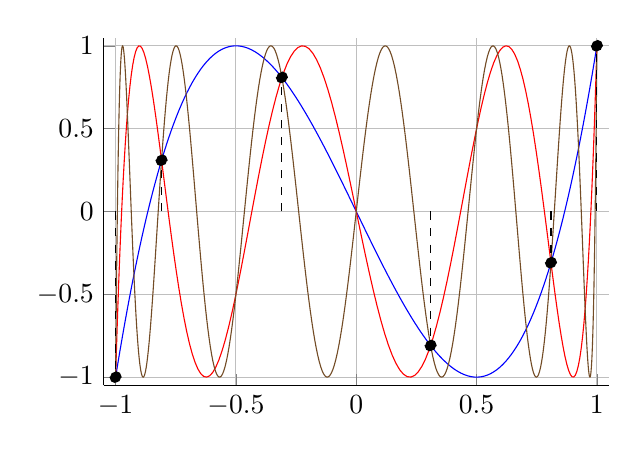
\begin{tikzpicture}
		\begin{axis}[%
			width=8cm, height=6cm,
			axis lines*=left,
			xmin=-1.0, xmax=1.0, ymin=-1.0, ymax=1.0,
			grid=major,
%			xtick = {-1,0,1},
%			ytick = {-1,0,1},
			clip marker paths=false,
			enlargelimits={abs=0.05},
			]%
			\addplot+[samples=200, domain=0:pi, no marks] ({cos(deg(x))}, {cos(3*deg(x))});% T_3
			\addplot+[samples=200, domain=0:pi, no marks] ({cos(deg(x))}, {cos(7*deg(x))});% T_7
			\addplot+[samples=500, domain=0:pi, no marks] ({cos(deg(x))}, {cos(13*deg(x))});% T_13
%			\addplot+[domain=-1:1, no marks, samples=200, black, dotted] {16*x^5 - 20*x^3 + 5*x};% T_5
			\addplot+[samples=6, domain=0:pi, ycomb, dashed, mark=*, black] ({cos(deg(x))}, {cos(3*deg(x))});% noeuds CGL de T_5
		\end{axis}
	\end{tikzpicture}
	\caption{Les polynômes $T_n$ (\protect\legenddash{s1}), $T_{2N - n}$ (\protect\legenddash{s2}) et $T_{2N + n}$ (\protect\legenddash{s3}) sont indiscernables aux n\oe uds CGL de $T_N$ (ici $n = 3$ et $N = 5$).}
	\label{fig:aliasing_cgl}
\end{figure}


\subsubsection{Évaluation}
Par la suite, nous serons amenés à évaluer à maintes reprises des sommes de la forme
\begin{equation}
	s_N = \sum_{n=0}^N \hat{s}_n T_n
	\label{eq:chebyshev_sum}
\end{equation}
en des points autres que les n\oe uds CGL.
Plutôt que de réécrire cette somme dans la base canonique de $\polyspace{N}$, il est intéressant de tirer parti de la relation \eqref{eq:chebyshev_recurrence}. 
En introduisant la suite récurrente
\begin{equation}
	b_n(x) = 
	\begin{cases}
	 0 & \text{\ si\ } n > N,   \\ 
	 \hat{s}_n - b_{n+2}(x) + 2x b_{n+1}(x) & \text{\ si\ } 0 \leq n \leq N,
	\end{cases}
\end{equation}
on obtient, pour $-1 \leq x \leq 1$,%
\def\px{}%{(x)}%
\begin{align*}
	s_N\px 
	&= \hat{s}_0 T_0\px + \hat{s}_1 T_1\px + \ldots + \hat{s}_{N-2} T_{N-2}\px + \hat{s}_{N-1} T_{N-1}\px + \hat{s}_N T_N\px, \\
	&= \hat{s}_0 T_0 \px
	+ \hat{s}_1 T_1 \px
	+ \ldots 
	+ \left(\hat{s}_{N-2} - b_{N}\px\right) T_{N-2} \px
	+ \left(\hat{s}_{N-1} - b_{N+1}\px + 2x b_{N}\px \right) T_{N-1}\px, \\
	&= \hat{s}_0 T_0 \px
	+ \hat{s}_1 T_1 \px
	+ \ldots 
	+ \left(\hat{s}_{N-3} - b_{N-1}\px\right) T_{N-3} \px
	+ b_{N-2}\px T_{N-2}\px, \\
	& \ldots\\
	&= \left( \hat{s}_0 - b_2\px \right) T_0\px + b_1\px T_1\px, \\
	&= \hat{s}_0 - b_2\px + b_1\px x,
\end{align*}
et enfin
\begin{equation}
	s_N(x) = b_0(x) - x b_1(x).
\end{equation}

L'exécution de cet algorithme de sommation --- proposé par Clenshaw \cite{clenshaw1955} --- requiert seulement $\bigO{N}$ opérations. %, ce qui le rend plus efficace que l'algorithme de Casteljau (dont la complexité est asymptotiquement quadratique). 
La sommation de Clenshaw est donc un moyen efficace et numériquement stable pour évaluer des séries de Chebyshev.


\subsubsection{Dérivation}
En posant $x = \cos\theta$, il vient, d'après \eqref{eq:chebyshev_trigo},
\begin{equation}
	T_n'(x) := \dfdx{T_n(x)}{x} = \frac{n \sin n\theta}{\sin \theta}.
\end{equation}
Ainsi, de l'identité $2 \cos n \theta \sin \theta = \sin(n+1)\theta - \sin(n-1)\theta$, on peut déduire la relation 
\begin{equation}
	2 T_n = \frac{T'_{n+1}}{n+1} - \frac{T'_{n-1}}{n-1} ,
	\label{eq:chebyshev_relation_deriv_3termes}
\end{equation}
pour $n \geq 2$.
\\
Soit $f \in \contdiff{k}\chebinterval$.
On approche la dérivée $k$-ième $\deriv{f}{k}$ de $f$ par la dérivée $k$-ième du polynôme d'interpolation $\interpolant{f}{N}$
\begin{equation}
	\interpderiv{f}{N}{k} := \deriv{ \left( \interpolant{f}{N} \right) }{k}.
	\label{eq:chebyshev_def_interpderiv}
\end{equation}
En général, les opérations de dérivation et d'interpolation ne commutent pas, \ie
\begin{equation}
	\interpderiv{f}{N}{k} \neq \interpolant{ \left( \deriv{f}{k} \right) }{N}.
\end{equation}

Les valeurs aux n\oe uds CGL de cette dérivée peuvent être exprimées comme une combinaison linéaire des valeurs de $f$ en ces mêmes n\oe uds
\begin{equation}
	\colvec{ 
		\interpderiv{f}{N}{k}(x_0) \\ 
		\vdots \\
		\interpderiv{f}{N}{k}(x_N)
		}
	=
	{\left( \mathbf{D}_N \right)}^k
	\colvec{ 
		f(x_0) \\ 
		\vdots \\
		f(x_N)
		},
	\label{eq:chebyshev_diff_at_cgl}
\end{equation}
où $\mathbf{D}_N$ est la matrice de différentiation \cite{canuto2006}
\def\cvsp{2.5ex}
\begin{equation}
	\left( \mathbf{D}_N \right)_{i,j} =
	\begin{cases}
	 \dfrac{2N^2 + 1}{6} & \text{\ si\ } i = j = 0,   \\[\cvsp]
	 -\dfrac{2N^2 + 1}{6} & \text{\ si\ } i = j = N,   \\[\cvsp]
	 -\dfrac{x_i}{2 \sin^2 \frac{i \pi}{N}} & \text{\ si\ } 0 < i = j < N, \\[\cvsp]
	 -\dfrac{(-1)^{i+j} \beta_i}{2 \beta_j \sin\frac{(i+j)\pi}{2N} \sin\frac{(i-j)\pi}{2N}} & \text{\ si\ } i \neq j.
	\end{cases}
	\label{eq:chebyshev_diff_matrix}
\end{equation}

Alternativement, il est intéressant de construire explicitement le polynôme dérivé $\interpderiv{f}{N}{k}$ comme une somme de la forme 
\begin{equation}
	\interpderiv{f}{N}{k} = \sum_{n=0}^{N-k} \deriv{\tilde{f}}{k}_n T_n.
\end{equation} 
Développer motivation\ldots
\par
La relation \eqref{eq:chebyshev_relation_deriv_3termes} implique que, pour tout $n \in \mathbb{N}$,
\begin{equation}
	2 (n + 1) \tilde{f}_{n+1} = \alpha_n \deriv{\tilde{f}}{1}_n - \deriv{\tilde{f}}{1}_{n+2}.
	\label{eq:chebyshev_prim_recurrence}
\end{equation}
Les coefficients $\deriv{\tilde{f}}{1}_n$ peuvent ainsi être calculés suivant la relation de récurrence
\begin{equation}
	\deriv{\tilde{f}}{1}_n = 
	\frac{1}{\alpha_n} \left( 2 (n + 1) \tilde{f}_{n+1} + \deriv{\tilde{f}}{1}_{n+2} \right).
	\label{eq:chebyshev_diff_recurrence}
\end{equation}
Plus généralement, les coefficients de Chebyshev de la dérivée $k$-ième vérifient
\begin{equation}
	\deriv{\tilde{f}}{k}_n = 
	\frac{1}{\alpha_n} \left( 2 (n + 1) \deriv{\tilde{f}}{k-1}_{n+1} + \deriv{\tilde{f}}{k}_{n+2} \right).
	\label{eq:chebyshev_diffp_recurrence}
\end{equation}

%On dispose ainsi d'un algorithme récursif pour construire les dérivées successives du polynôme $\interpolant{f}$. 
Cette méthode + FFT permet d'évaluer les dérivées aux n\oe uds CGL pour $\bigO{N + N \log N} = \bigO{N \log N}$, qui est asymptotiquement (au-delà de $N \approx 16$) plus efficace que le produit matrice-vecteur \eqref{eq:chebyshev_diff_at_cgl} ($\bigO{N^2}$).
\par
Toutefois, comme l'ont fait remarquer Wengle et Seinfeld \cite{wengle1978}, l'algorithme récursif \eqref{eq:chebyshev_diffp_recurrence} peut amplifier les erreurs d'arrondi commises sur les plus petits coefficients $\deriv{\hat{f}}{k-1}_{n}$ et ainsi compromettre la précision de \emph{tous} les coefficients $\deriv{\hat{f}}{k}_{n}$. 
Un moyen simple de remédier à ce problème consiste à mettre à zéro les coefficients $\deriv{\hat{f}}{k-1}_{n}$ inférieurs en valeur absolue à un seuil donné, choisi en fonction de la précision machine $\epsilon_M$. 
(Un seuil égal à $10 \epsilon_M$ semble être un bon choix \textit{(détailler\ldots)}.)

%L'étude menée jusqu'ici concerne l'approximation de fonctions d'une variable par des séries de Chebyshev. 
%Les résultats présentés se généralisent aux fonctions de plusieurs variables en utilisant les polynômes de Chebyshev en produit tensoriel. 
%On se limitera ici aux fonctions de deux variables, utiles pour représenter des surfaces. 
%Ainsi, une fonction $f$ continue sur $\chebinterval^2$ admet un développement en série de Chebyshev
%\begin{equation}
%	f(u,v) = \sum_{m=0}^{\infty} \sum_{n=0}^{\infty} \hat{f}_{m,n} T_m(u) T_n(v),
%\end{equation}
%dont la somme partielle
%\begin{equation}
%	\truncseries{f}{MN} (u,v) = \sum_{m=0}^{M} \sum_{n=0}^{N} \hat{f}_{m,n} T_m(u) T_n(v)
%\end{equation}
%converge uniformément vers $f$ sur $\chebinterval^2$.

%fonctions d'une variable
%\begin{itemize}
%	\item orthogonalité $\Rightarrow$ aspect multirésolution, élévation/réduction de degré directe et quasi-optimale (d'ailleurs utilisé en CAO \cite{lachance1988})
%	\item série tronquée $\truncseries{f}{N}$, erreur de troncature, précision spectrale :\\
%si $f \in \contdiffp(\chebinterval)$, alors $\max_{\chebinterval} \left| \truncseries{f}{N} - f \right| = \bigO{N^{1-p}}$ lorsque $N \to \infty$ \cite[Théorème 5.14]{mason2002} (illustration convergence exponentielle pour $f$ analytique et décroissance exponentielle des $\hat{f}_n$)
%	\item interpolant $\interpolant{f}{N}$, erreur d'aliasing
%	\item CGL $\to$ DCT, transformation rapide
%\end{itemize}
%généralisation à plusieurs variables (produit-tensoriel)


\begin{figure}%[!htp]
\centering%
\hspace*{\fill}%
\subbottom[Erreur d'approximation par le polynôme $\interpderiv{f}{N}{k}$.]{%
\begin{tikzpicture}%
\begin{semilogyaxis}[
	width=6.7cm, height=6cm,
	xmin=0, xmax=100,
	ymin=1.0e-16, ymax=1.0e2,
	grid=both,
	axis x line*=bottom,
	axis y line*=left,
	xlabel={$N\vphantom{n}$},
	ylabel={\small $\norminf{\interpderiv{f}{N}{k} - \deriv{f}{k}} \norminf{\deriv{f}{k}}^{-1}$},
	xtick distance=25,
	legend pos=north east,
	legend style={font=\small},
	cycle list shift=-1
	]%
	%\addplot+[dashed, color=black, no marks, very thick][domain=40:60] {0.5*exp(-0.57*x)} node[pos=0.5, anchor=north east, font=\footnotesize, inner sep=1pt] {$1.8^{-N}$};%
	\addplot+[dashed, color=black, no marks, very thick][domain=40:60] {0.5*exp(-0.57*x)};%
	\addlegendentry{$1.8^{-N}$}
	\pgfplotsinvokeforeach{1,...,3}{
		\addplot+ table[x index=0, y index=#1] {figures/data/convergence_DNkf.dat};%
	}
\end{semilogyaxis}%
\end{tikzpicture}%
\label{subfig:spectral_convergence_Linf}%
}%
\hspace{4mm}%
%\hfill%
\subbottom[Spectre des coefficients de Chebyshev.]{% du polynôme $\interpderiv{f}{80}{k}$.]{%
\begin{tikzpicture}%
\begin{semilogyaxis}[%
	width=6.7cm, height=6cm,
	xmin=0, xmax=100,
	ymin=1.0e-16, ymax=1.0e2,
	grid=major,
	axis y line*=right,
	axis x line*=bottom,
	xlabel={$n\vphantom{N}$},
	ylabel={},
	ylabelv right={$\left | \tilde{f}_n^{(k)} \right |$},
	ylabel near ticks, 
	yticklabel pos=right,
	yticklabels={\empty},
	xtick distance=25,
	legend pos=north east,
	legend style={font=\small},
	cycle list shift=-1
	]%
%	\addplot+[dashed, color=black, no marks, very thick][domain=40:60] {0.5*exp(-0.57*x)} node[pos=0.5, anchor=north east, font=\footnotesize, inner sep=1pt] {$1.8^{-n}$};
	\addplot+[dashed, color=black, no marks, very thick][domain=40:60] {0.5*exp(-0.57*x)};
	\addlegendentry{$1.8^{-n}$}
	\pgfplotsinvokeforeach{0,...,2}{
		\addplot+[only marks] table[x expr=\coordindex, y index=#1] {figures/data/coef_DNkf.dat};%
	}
\end{semilogyaxis}%
\end{tikzpicture}%
\label{subfig:spectral_convergence_coef}%
}
\hspace*{\fill}%
\caption{Décroissance exponentielle de l'erreur d'approximation et des coefficients de Chebyshev pour la fonction analytique $f : x \mapsto e^{\sin 3 x^3}$ et ses dérivées $\deriv{f}{k}$ ($k = 0 (\protect\legendsquare{s1}), 1 (\protect\legenddot{s2}), 2 (\protect\legendtriangle{s3})$).}%
\label{fig:spectral_convergence}%
\end{figure}

%\paragraph{Représentation de courbes et de surfaces.}
%Afin de représenter des courbes et surfaces plongées dans l'espace euclidien $\mathbb{R}^3$ on développe chaque composante de la paramétrisation à l'aide d'une série de Chebyshev.
%Soit une courbe décrite par la paramétrisation $\bg : \chebinterval \to \mathbb{R}^3$. On notera alors
%\begin{equation}
%	\bg(t) = \sum_{n=0}^{\infty} \hat{\bg}_{n} T_n(t).
%\end{equation}
%surface $\bs : \chebinterval^2 \to \mathbb{R}^3$
%\begin{equation}
%	\truncseries{\bs}{MN}(u,v) = \sum_{m=0}^{M} \sum_{n=0}^{N} \hat{\bs}_{mn} T_m(u) T_n(v).
%\end{equation}

\subsubsection{Intégration}
Intégrale indéfinie/Primitive de $\interpolant{f}{N}$ qui s'annule en $-1$
\begin{equation}
	\interpprim{f}{N} := x \mapsto \int_{-1}^{x} \interpolant{f}{N}(t) \dx{t}
\end{equation}
c'est un polynome de degré $N+1$
\begin{equation}
	\interpprim{f}{N} = \sum_{n=0}^{N+1} \prim{\tilde{f}}{1}_n T_n.
\end{equation}

\eqref{eq:chebyshev_prim_recurrence} implique 
\begin{equation}
	\prim{\tilde{f}}{1}_n = \frac{\alpha_n \tilde{f}_{n-1} - \tilde{f}_{n+1}}{2n},
\end{equation}
pour $n \geq 1$ et, puisque $\interpprim{f}{N}(-1) = 0$, on a
\begin{equation}
	\prim{\tilde{f}}{1}_0 = - \sum_{n=1}^{N+1} (-1)^n \prim{\tilde{f}}{1}_n.
\end{equation}

\begin{equation}
	\int_{-1}^{x} f(t) \dx{t} 
	\approx \interpprim{f}{N}(x).
\end{equation}
En particulier,
\begin{equation}
	\int_{-1}^{1} f(t) \dx{t} 
	\approx 
	\interpprim{f}{N}(1)
	=
	\sum_{\mathclap{\substack{n = 0\\n \text{ pair}}}}^{N} \frac{2 \tilde{f}_n}{1 - n^2},
\end{equation}
et
\begin{equation}
	\left| \int_{-1}^{1} f(x) \dx{x} - \interpprim{f}{N}(1) \right|
	\approx
	\left|\frac{2 \tilde{f}_{N}}{1 - N^2}\right|.
\end{equation}
%La \eqref{eq:chebyshev_relation_deriv_3termes} implique
%\begin{equation}
%\int_{-1}^{1} T_n(x) \dx{x} = 
%\begin{cases}
%		0 \text{\ si\ } n \text{\ est impair,} \\
%		%\frac{1}{n+1} - \frac{1}{n-1} = \frac{2}{1 - n^2} \text{\ si\ } n \text{\ est pair.}
%		\frac{1}{n+1} - \frac{1}{n-1} \text{\ si\ } n \text{\ est pair.}
%	\end{cases}
%\end{equation}
%Et donc
%\begin{equation}
%	\int_{-1}^{1} f(x) \dx{x} 
%	\approx \int_{-1}^{1} \interpolant{f}{2N}(x) \dx{x}  
%	= \sum_{n=0}^{N}\frac{2 \tilde{f}_{2n}}{1 - 4n^2}.
%\end{equation}
%et
%\begin{equation}
%	\left| \int_{-1}^{1} f(x) \dx{x} - \int_{-1}^{1} \interpolant{f}{2N}(x) \dx{x} \right|
%	\approx
%	\left|\frac{2 \tilde{f}_{2N}}{1 - 4N^2}\right|.
%\end{equation}

Clenshaw-Curtis (quadrature imbriquée/adaptative)?\\
calcul longueur de courbe/aire de surface (approximation, l'intégrande n'est généralement pas polynomiale)

\begin{equation}
	\int_{-1}^{1} \int_{-1}^{1} g(u,v) \dx{u} \dx{v}
	\approx 
	\interpprim{\,g}{M,N}(1,1)
	=
	\sum_{\mathclap{\substack{m = 0\\m \text{ pair}}}}^{M}
	\;\;
	\sum_{\mathclap{\substack{n = 0\\n \text{ pair}}}}^{N} 
	\frac{4 \tilde{g}_{m,n}}{(1 - m^2)(1 - n^2)},
\end{equation}

\begin{align}
	\left| \int_{-1}^{1} \int_{-1}^{1} g(u,v) \dx{u}\dx{v} - \interpprim{\,g}{M,N}(1,1) \right|
	\approx
	\sum_{\mathclap{\substack{m = 0\\m \text{ pair}}}}^{M} \left| \frac{4 \tilde{g}_{m,N}}{(1 - m^2)(1 - N^2)} \right| \nonumber\\ + 
	\sum_{\mathclap{\substack{n = 0\\n \text{ pair}}}}^{N} \left| \frac{4 \tilde{g}_{M,n}}{(1 - M^2)(1 - n^2)} \right| \nonumber\\ +
	\left| \frac{4 \tilde{g}_{M,N}}{(1 - M^2)(1 - N^2)} \right|.
\end{align}

%\begin{figure}
%\centering
%\begin{tikzpicture}
%\invertcolormap{RdBu}
%\begin{groupplot}[
%	group style={group size=5 by 3},
%	height=3.6cm,
%	width=3.6cm,
%	unit vector ratio*=1 1 1,
%	domain=0:pi,
%	y domain=0:pi, 
%	xmin=-1, xmax=1,
%	ymin=-1, ymax=1,
%	zmin=-1, zmax=1,
%	axis lines*=left,
%	xtick={-1,0,1}, 
%	ytick={-1,0,1}, 
%	ztick={-1,0,1}, 
%	view={-37.5}{30},
%	grid=major]
%	\pgfmathsetmacro\mmax{3}
%	\pgfmathsetmacro\nmax{4}
%	\pgfmathsetmacro\mn{(\mmax+1)*(\nmax+1)}
%	\pgfplotsinvokeforeach{1,...,\mn}{
%		\nextgroupplot[
%			xticklabels=\empty,
%			yticklabels=\empty,
%			zticklabels=\empty
%			]
%		\pgfmathtruncatemacro\nn{\currentcolumn-1}
%    	\pgfmathtruncatemacro\mm{\currentrow-1}
%    	\addplot3 graphics [
%			points={
%			(0,0,0) => (116.5,225-108.5)
%			(1,0,0) => (165.5,225- 90.5)
%			(0,1,0) => ( 78.5,225- 85.5)
%			(0,0,1) => (116.5,225- 58.0)
%			}] {figures/T_\mm_\nn.png};
%	}
%\end{groupplot}
%\end{tikzpicture}
%\end{figure}

\def\degru{6}
\def\degrv{5}
\def\uvsize{32mm}
\def\fracaxeoffset{0.1}
\def\fracduv{0.2}
\def\distanceaxe{1.7*\MajorTickLength}
\colorlet{uvbgcolor}{white!92!black}
\begin{figure}%
\centering%
\hspace*{\fill}%
\subbottom[Grille CGL $uv$.]{%
\begin{tikzpicture}[
	point/.style={circle, fill=black, scale=0.22},
	bigpoint/.style={circle, fill=black, scale=0.33},
	isouv/.style={dotted, line width=0.5pt},
	tick/.style={line width=0.5pt},
	axe/.style={-stealth, tick},
	label/.style={font=\small, inner sep=1.5pt},
	vector/.style={-latex', very thick},
	ticklabel/.style={label, inner sep=\MajorTickLength}]
%
\coordinate (uvnorth) at (0,{0.5*\parampatchimageheight});
\coordinate (uvsouth) at (0,{-0.5*\parampatchimageheight});
\node at (uvnorth) {};
\node at (uvsouth) {};
%
\foreach \j in {0,...,\degrv} {
	\foreach \i in {0,...,\degru} {
		\coordinate (uv\i\j) at (
			{0.5*cos(\i*pi/\degru r)*\uvsize},
			{0.5*cos(\j*pi/\degrv r)*\uvsize}
		);
	}
}
%
\draw[fill=uvbgcolor, semithick] 
(uv00) -- (uv\degru0) -- (uv\degru\degrv) -- (uv0\degrv) -- cycle;
%
\foreach \j in {0,...,\degrv} {
	\foreach \i in {0,...,\degru} {
		\node[point] at (uv\i\j) {};
	}
}
\foreach \i in {0,...,\degru} {\draw[isouv] (uv\i0) -- (uv\i\degrv);}
\foreach \j in {0,...,\degrv} {\draw[isouv] (uv0\j) -- (uv\degru\j);}
%
% Axes
\coordinate (o) at ({-0.5*\uvsize-\distanceaxe},{-0.5*\uvsize-\distanceaxe});
\draw[axe] (o) -- ++ ({(1.0+\fracaxeoffset)*\uvsize+\distanceaxe},0) node [label, anchor=west] {$u$};
\draw[axe] (o) -- ++ (0,{(1.0+\fracaxeoffset)*\uvsize+\distanceaxe}) node [label, anchor=south] {$v$};
% Ticks
\gettikzxy{(o)}{\ox}{\oy}
\foreach \i in {-1,0,1} {
	\draw[tick] ({0.5*\i*\uvsize},{\oy}) -- ({0.5*\i*\uvsize},{\oy+\MajorTickLength});
	\node[anchor=north, ticklabel] at ({0.5*\i*\uvsize},\oy) {$\i$};
}
\foreach \j in {-1,0,1} {
	\draw[tick] ({\ox},{0.5*\j*\uvsize}) -- (\ox+\MajorTickLength,{0.5*\j*\uvsize});
	\node[anchor=east, ticklabel] at (\ox,{0.5*\j*\uvsize}) {$\j$};
}
%
\def\i{4}
\def\j{3}
\node[label, fill=uvbgcolor, rectangle, rounded corners=1ex, label, anchor=north, inner sep=0.5pt, yshift=-1.5pt] at (uv\i\j) {$(u_i,v_j)$};
\draw[vector, red] (uv\i\j) -- ++ ({\fracduv*\uvsize},0);
\draw[vector, blue] (uv\i\j) -- ++ (0,{\fracduv*\uvsize});
\node[bigpoint] at (uv\i\j) {};
\end{tikzpicture}%
\label{subfig:cgl_grid_uv}%
}%
\hfill%
\subbottom[Grille CGL $xyz$.]{
\def\parampatchimagewidth{80mm}
\def\parampatchimageheight{0.75*\parampatchimagewidth}
\begin{tikzpicture}[
	x=\parampatchimagewidth,
	y=\parampatchimageheight,
	im/.style={anchor=south west, inner sep=0pt},
	bigpoint/.style={circle, fill=black, scale=0.33},
	axe/.style={-stealth, line width=0.5pt},
	label/.style={font=\small, inner sep=1.5pt},
	vector/.style={-latex', very thick}]
\coordinate (a) at (0,0);
{\transparent{\parampatchshadowtransparency}\node[im] (shadow) at (a) {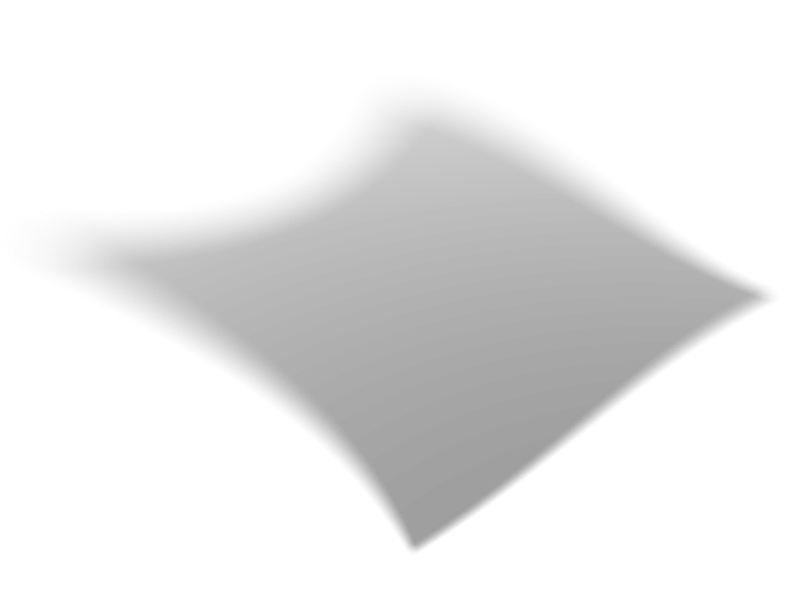
\includegraphics[width=\parampatchimagewidth]{figures/parametric_patch_shadow}};}
% trièdre
\def\scaletriedre{0.85}
\coordinate (o) at (0.20309802889823914 ,  0.26374515891075134);
\coordinate (x) at (0.30103224515914917 ,  0.14841561019420624);
\coordinate (y) at (0.3310101628303528 ,  0.3642595410346985);
\coordinate (z) at (0.17395645380020142 ,  0.43496546149253845);
\draw[axe] (o) -- ($(o)!\scaletriedre!(x)$) node[label, anchor=west] {$x$};
\draw[axe] (o) -- ($(o)!\scaletriedre!(y)$) node[label, anchor=west] {$y$};
\draw[axe] (o) -- ($(o)!\scaletriedre!(z)$) node[label, anchor=south] {$z$};
%
\node[im] at (a) {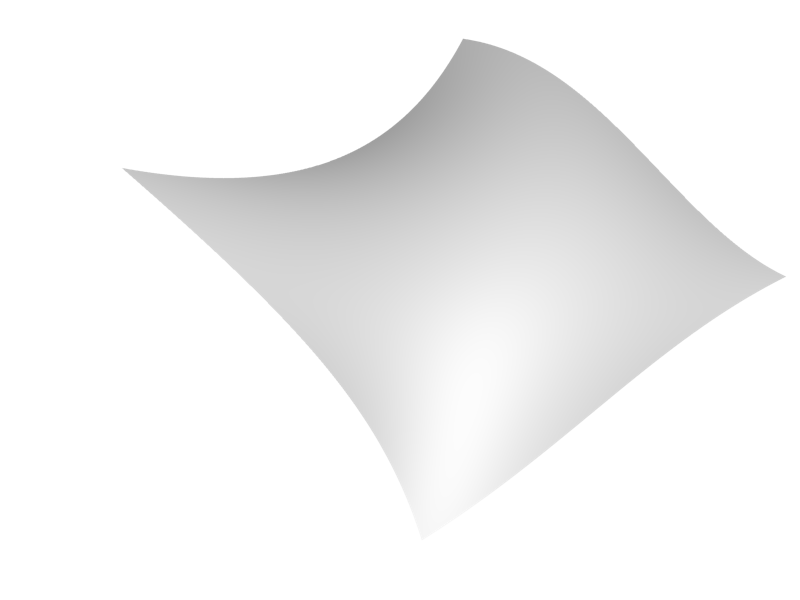
\includegraphics[width=\parampatchimagewidth]{figures/parametric_patch_surface}};
\node[im] at (a) {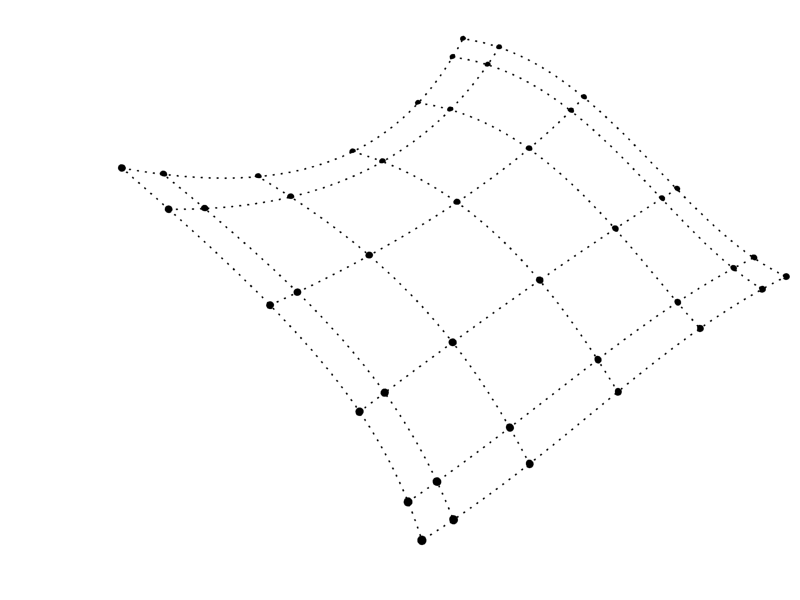
\includegraphics[width=\parampatchimagewidth]{figures/parametric_patch_cgl_grid}};
\node[im] at (a) {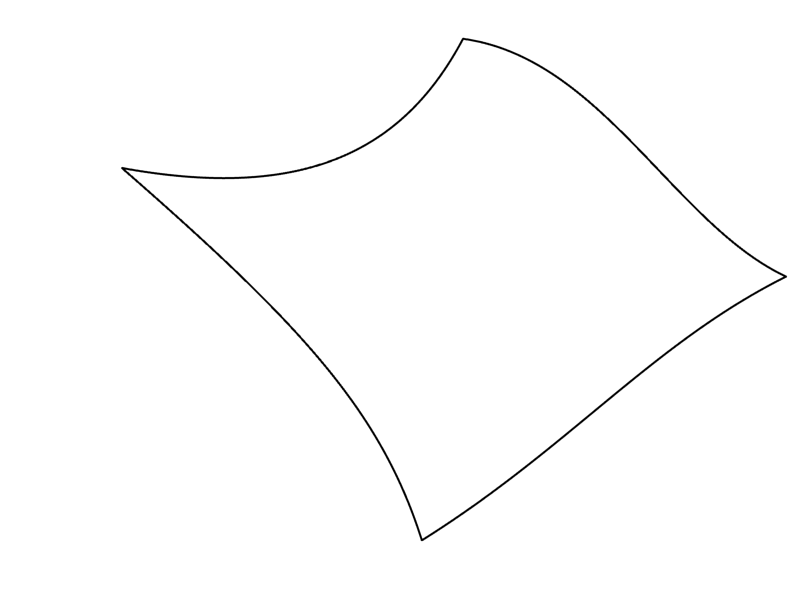
\includegraphics[width=\parampatchimagewidth]{figures/parametric_patch_border}};
% vecteurs
\def\scalevectors{0.99}
\coordinate (s) at (0.5657749772071838, 0.4292657971382141);
\coordinate (u) at (0.6539148092269897, 0.5149791240692139);
\coordinate (v) at (0.506170392036438, 0.5304208993911743);
\coordinate (n) at (0.5878586769104004, 0.5399532318115234);
\draw[vector, red] (s) -- ($(s)!\scalevectors!(u)$) node[label, anchor=north west, xshift=-2pt] {$\bx_u$};
\draw[vector, blue] (s) -- ($(s)!\scalevectors!(v)$) node[label, anchor=east, yshift=-1pt] {$\bx_v$};
\draw[vector, black] (s) -- ($(s)!\scalevectors!(n)$) node[label, anchor=south] {$\unv$};
\node [bigpoint] at (s) {};
\node [label, anchor=north, inner sep=7pt] at (s) {$\bx_{i,j}$};
\end{tikzpicture}%
%\begin{tikzpicture}[
%	im/.style={anchor=north west, inner sep=0pt},
%	bigpoint/.style={circle, fill=black, scale=0.33},
%	axe/.style={-stealth, line width=0.5pt},
%	label/.style={font=\small, inner sep=1.5pt},
%	vector/.style={-latex', very thick}]
%\coordinate (a) at (0,0);
%{\transparent{\parampatchshadowtransparency}\node[im] (shadow) at (a) {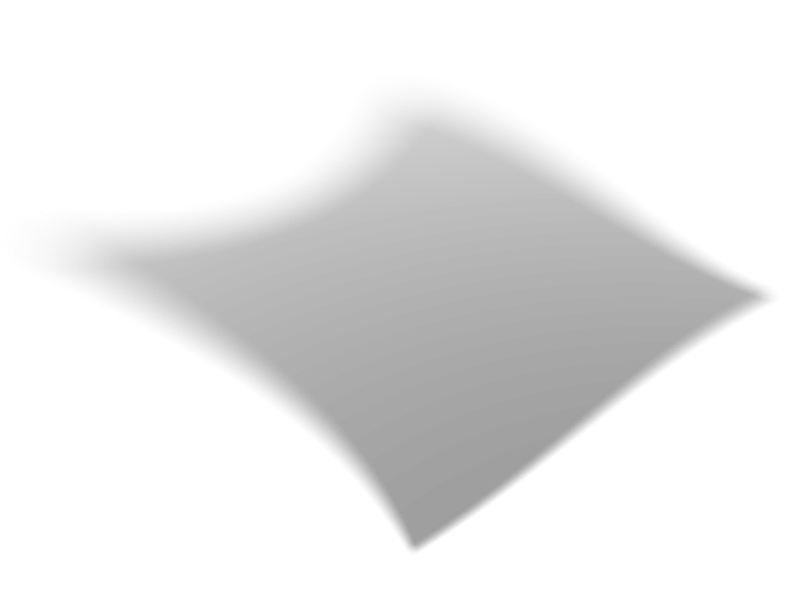
\includegraphics[width=\parampatchimagewidth]{figures/parametric_patch_shadow}};}
%% trièdre
%\def\scaletriedre{0.85}
%\coordinate (o) at ([xshift=14.90mm, yshift=-45.52mm]a);%(16.38mm, -44.12mm);
%\coordinate (x) at ([xshift=22.70mm, yshift=-52.72mm]a);%(26.68mm, -48.84mm);
%\coordinate (y) at ([xshift=25.32mm, yshift=-39.38mm]a);%(24.22mm, -37.05mm);
%\coordinate (z) at ([xshift=12.40mm, yshift=-32.25mm]a);%(13.92mm, -33.98mm);
%\draw[axe] (o) -- ($(o)!\scaletriedre!(x)$) node[label, anchor=west] {$x$};
%\draw[axe] (o) -- ($(o)!\scaletriedre!(y)$) node[label, anchor=west] {$y$};
%\draw[axe] (o) -- ($(o)!\scaletriedre!(z)$) node[label, anchor=south] {$z$};
%%
%\node[im] at (a) {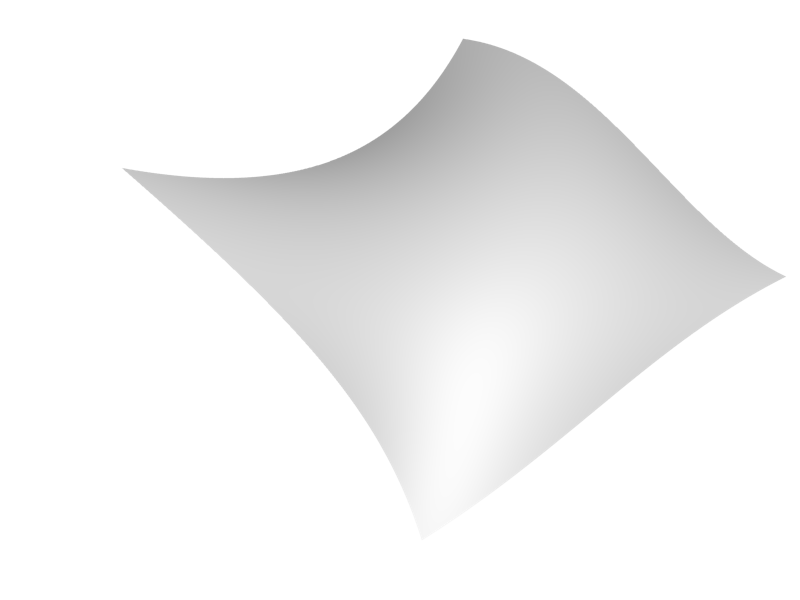
\includegraphics[width=\parampatchimagewidth]{figures/parametric_patch_surface}};
%\node[im] at (a) {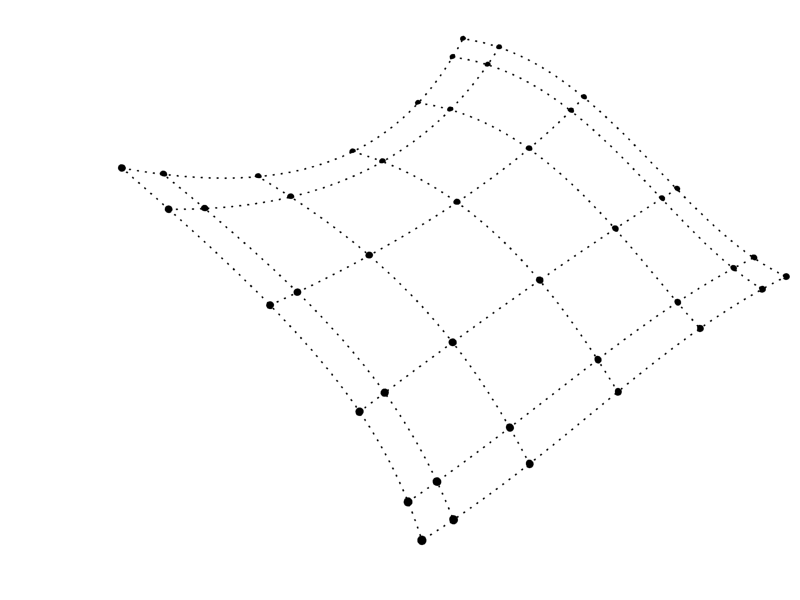
\includegraphics[width=\parampatchimagewidth]{figures/parametric_patch_cgl_grid}};
%\node[im] at (a) {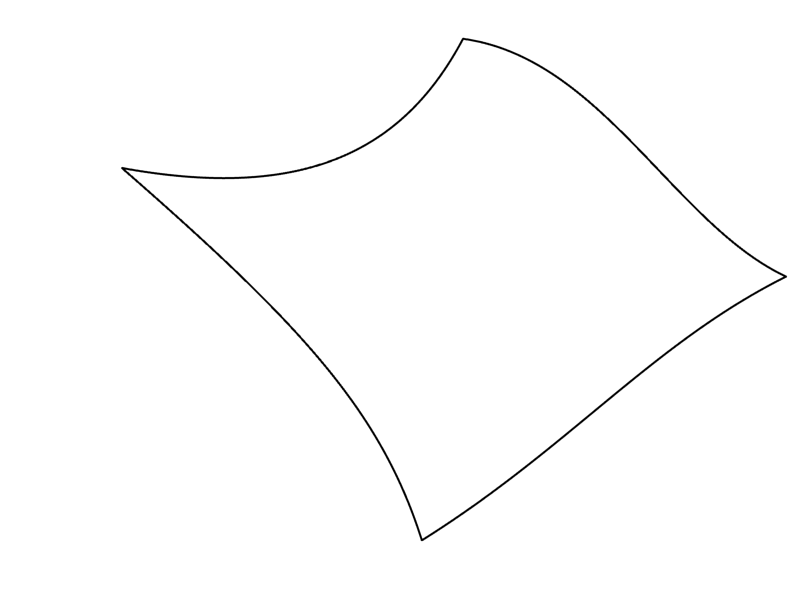
\includegraphics[width=\parampatchimagewidth]{figures/parametric_patch_border}};
%% vecteurs
%\def\scalevectors{0.99}
%\coordinate (s) at ([xshift=45.29mm, yshift=-34.21mm]a);
%\coordinate (u) at ([xshift=52.26mm, yshift=-29.14mm]a);
%\coordinate (v) at ([xshift=40.55mm, yshift=-28.25mm]a);
%\coordinate (n) at ([xshift=47.02mm, yshift=-27.62mm]a);
%\draw[vector, red] (s) -- ($(s)!\scalevectors!(u)$) node[label, anchor=north west, xshift=-2pt] {$\bx_u$};
%\draw[vector, blue] (s) -- ($(s)!\scalevectors!(v)$) node[label, anchor=east, yshift=-1pt] {$\bx_v$};
%\draw[vector, black] (s) -- ($(s)!\scalevectors!(n)$) node[label, anchor=south] {$\unv$};
%\node [bigpoint] at (s) {};
%\node [label, anchor=north, inner sep=7pt] at (s) {$\bx_{i,j}$};
%\end{tikzpicture}%
\label{subfig:cgl_grid_xyz}%
}
\hspace*{\fill}%
\caption{Grille CGL.}%
\label{fig:cgl_grid}%
\end{figure}



\section{Intégration temporelle}%{Discrétisation temporelle}
\begin{itemize}
	\item champ de vitesse connu : intégration classique, schéma explicite (Euler, RK)
	\item vitesse normale connue : approximation EdS
	\begin{itemize}
		\item calcul dérivées par différentiation spectrale
		\item calcul normale et composante tangentielle
%		\item non-linéarités $\to$ aliasing, peut causer instabilité \cite{rahimian2015}
	\end{itemize}
%	\item auto-intersections
%	\begin{itemize}
%		\item globales (traitées au chapitre 3)
%		\item locales \cite{farouki1986}
%	\end{itemize}
\end{itemize}


\section{Instabilités\ldots}
\label{sec:instabilites}
\begin{itemize}
	\item non-linéarités $\to$ aliasing, peut causer instabilité \cite{rahimian2015}, atténuation : sur-échantillonnage, filtrage
	\item auto-intersections
	\begin{itemize}
		\item globales (traitées au \autoref{chap:multi_patch})
		\item locales \cite{farouki1986} (détection, résolution?)
	\end{itemize}
\end{itemize}
